% !TeX program = xelatex
% !TeX encoding = UTF-8
% !TeX TXS-program:compile = txs:///xelatex | txs:///xelatex
\documentclass[aspectratio=169, table, 12pt]{beamer}

% Preamble bersama seluruh slide mata kuliah ini.
% Dipanggil dari slides/sessionXX/sessionXX.tex tepat sesudah baris
% \documentclass[aspectratio=169, table, 12pt]{beamer}
% Paket tambahan yang hanya dibutuhkan satu sesi ditulis di berkas sesi itu.

\usepackage{colortbl}
\usepackage{xcolor}
\usepackage{listings}
\usepackage{tabularx}
\usepackage{booktabs}
\usepackage{tikz}
\usepackage{pgfplots}
\usepackage{fontspec}
\usepackage[english,bahasai]{babel}
\pgfplotsset{compat=1.18}
\usetikzlibrary{arrows.meta, positioning, calc, fit, shapes.geometric,
  shapes.multipart, backgrounds, matrix, chains, trees}

\makeatletter
\def\input@path{{../theme/}}
\makeatother
\graphicspath{{../theme/}{../../figures/}}
% Stub symlink Windows memakai tema cadangan sampai aset institusi tersedia.
\IfFileExists{../theme/beamerthemePradita.sty}{%
  \usetheme{Pradita}
}{%
  \usetheme{Madrid}
  \setmainfont{TeX Gyre Heros}
  \setsansfont{TeX Gyre Heros}
  \setbeamertemplate{navigation symbols}{}
}

\definecolor{praditagreen}{RGB}{37, 113, 71}
\setbeamercolor{structure}{fg=praditagreen}
\setbeamercolor{palette primary}{bg=praditagreen,fg=white}
\setbeamercolor{palette secondary}{bg=praditagreen!80!black,fg=white}
\setbeamercolor{palette tertiary}{bg=praditagreen!60!black,fg=white}
\setbeamerfont{frametitle}{size=\large}
\setbeamertemplate{caption}[numbered]

% Ukuran header mengikuti teks agar judul panjang tidak menabrak logo.
\setbeamercolor{frametitle}{bg=white,fg=black}
\setbeamertemplate{frametitle}{%
  \begin{beamercolorbox}[wd=\paperwidth,sep=0.2cm]{frametitle}
    \begin{minipage}[c]{0.77\paperwidth}
      \raggedright\fontsize{16}{18}\selectfont\bfseries\insertframetitle
      \ifx\insertframesubtitle\empty\else
        \par\small\mdseries\insertframesubtitle
      \fi
    \end{minipage}\hfill
    \begin{minipage}[c]{0.15\paperwidth}
      \IfFileExists{../theme/classFiles/logo_universitas.png}{%
        
\includegraphics[width=\linewidth]{../theme/classFiles/logo_universitas.png}%
      }{}
    \end{minipage}
  \end{beamercolorbox}
}
\setbeamertemplate{footline}{%
  \ifnum\value{framenumber}>1
    \begin{beamercolorbox}[wd=\paperwidth,ht=0.35cm,dp=0.15cm,
      leftskip=0.3cm,rightskip=0.3cm]{palette primary}
      \footnotesize\bfseries\insertframenumber/\inserttotalframenumber
      \hfill IT40513
    \end{beamercolorbox}
  \fi
}
\DeclareRobustCommand{\berkas}[1]{\path{#1}}

% Tema membuat garis tabel berwarna putih. Dikembalikan agar tabel terbaca.
\arrayrulecolor{black}
\setlength{\arrayrulewidth}{0.5pt}

\lstdefinelanguage{yaml}{
  basicstyle=\ttfamily\scriptsize,
  keywordstyle=\color{blue}\bfseries,
  commentstyle=\color{gray}\itshape,
  stringstyle=\color{red},
  showstringspaces=false,
  breaklines=true,
  frame=lines,
  numbers=none,
  backgroundcolor=\color{lightgray!10},
  tabsize=2,
  morecomment=[l]{\#}
}

\lstdefinelanguage{json}{
  basicstyle=\ttfamily\scriptsize,
  stringstyle=\color{red},
  commentstyle=\color{gray},
  breaklines=true,
  showstringspaces=false,
  tabsize=2,
  numbers=none,
  frame=lines,
  backgroundcolor=\color{lightgray!10},
  string=[s]{"}{"}
}

\lstdefinelanguage{bash}{
  keywords={},
  basicstyle=\ttfamily\scriptsize,
  ndkeywords={docker, kubectl, helm, curl, git, terraform},
  ndkeywordstyle=\color{purple}\bfseries,
  sensitive=true,
  commentstyle=\color{gray},
  numbers=none,
  breaklines=true,
  frame=lines,
  backgroundcolor=\color{lightgray!10},
  tabsize=2,
  comment=[l]{\#},
  showstringspaces=false
}

\lstdefinelanguage{http}{
  keywords={GET, POST, PUT, PATCH, DELETE, HEAD, OPTIONS, HTTP},
  basicstyle=\ttfamily\scriptsize,
  keywordstyle=\color{blue}\bfseries,
  sensitive=true,
  numbers=none,
  breaklines=true,
  frame=lines,
  backgroundcolor=\color{lightgray!10},
  tabsize=2,
  showstringspaces=false
}

\subtitle{IT40513 · Enterprise Architecture \& Digital Blueprint}
\author{\textbf{Alfa Yohannis}}


% Sampul membatasi judul di panel putih tema rujukan Pradita.
\setbeamertemplate{title page}{%
  \begin{tikzpicture}[remember picture,overlay]
    \node[anchor=north west,inner sep=0pt,text width=8.8cm]
      at ([xshift=1cm,yshift=-3.15cm]current page.north west) {%
        {\small\insertsubtitle\par}\vspace{0.25cm}
        \resizebox{8.8cm}{!}{\begin{minipage}{12cm}
          \raggedright\color{praditagreen}\bfseries\inserttitle
        \end{minipage}}
      };
    \node[anchor=south west,inner sep=0pt]
      at ([xshift=1cm,yshift=1.65cm]current page.south west)
      {\small\insertdate};
    \node[anchor=west,inner sep=0pt,text=white]
      at ([xshift=0.8cm,yshift=0.75cm]current page.south west)
      {\small\insertauthor};
  \end{tikzpicture}
}


% Batasi kedua dimensi gambar agar diagram bersama tetap berada pada slide.
\newsavebox{\eafigbox}
\newcommand{\eadiagram}[1]{%
  \sbox{\eafigbox}{\resizebox{0.94\textwidth}{!}{\input{#1}}}%
  \ifdim\dimexpr\ht\eafigbox+\dp\eafigbox\relax>0.64\textheight
    \resizebox{!}{0.64\textheight}{\usebox{\eafigbox}}%
  \else
    \usebox{\eafigbox}%
  \fi
}


\title{\Huge Kerangka Arsitektur:\\ \vspace{10pt} TOGAF, Zachman, SPBE}
\date{Pertemuan 02}

\begin{document}

\frame{\titlepage}

\begin{frame}
  \frametitle{Isi Pertemuan}
  \vspace{14pt}
  \begin{columns}[t]
    \column{0.5\textwidth}
    {\small\tableofcontents[sections={1-3}]}

    \column{0.5\textwidth}
    {\small\tableofcontents[sections={4-6}]}
  \end{columns}
\end{frame}

\begin{frame}{\hfill}
  \centering
  \Huge{\textbf{Tiga dokumen, satu\\organisasi: mengapa\\tidak dapat\\dibandingkan?}}
\end{frame}

\section{Tujuan dan Konteks}

\begin{frame}{\hfill}
  \centering
  \Huge{\textbf{Tujuan dan Konteks}}
\end{frame}

\begin{frame}{{\Large Tujuan Pembelajaran}}
  \vspace{10pt}
  \begin{itemize}
    \item Menjelaskan struktur TOGAF Standard edisi ke-10 dan urutan fase ADM (\textit{Architecture
          Development Method}).
    \item Membandingkan TOGAF, Zachman Framework, dan Arsitektur SPBE (Sistem Pemerintahan Berbasis
          Elektronik) dari sisi tujuan, cakupan, dan cara pakai.
    \item Menyusun peta pemangku kepentingan beserta \textit{concern} dan ruang lingkup kerja
          arsitektur.
  \end{itemize}
\end{frame}

\begin{frame}{{\Large Tiga Dokumen, Tiga Akibat}}
  \vspace{6pt}
  \small
  \begin{itemize}
    \item Dokumen vendor SIMRS (Sistem Informasi Manajemen Rumah Sakit): diagram server dan basis data.
    \item Dokumen konsultan ERP (\textit{Enterprise Resource Planning}) keuangan: peta proses dan daftar
          laporan.
    \item Dokumen tim internal: daftar aplikasi dengan kolom yang berbeda lagi.
    \item Akibatnya, dokumen sulit dibandingkan, kelengkapannya sulit diperiksa, dan hasil kerja sulit
          dipakai ulang.
    \item Kerangka kerja arsitektur menyediakan kosakata, susunan isi, dan urutan kerja yang disepakati
          bersama.
  \end{itemize}
\end{frame}

\begin{frame}{{\Large Diagram Konsep Bab 2}}
  \centering
  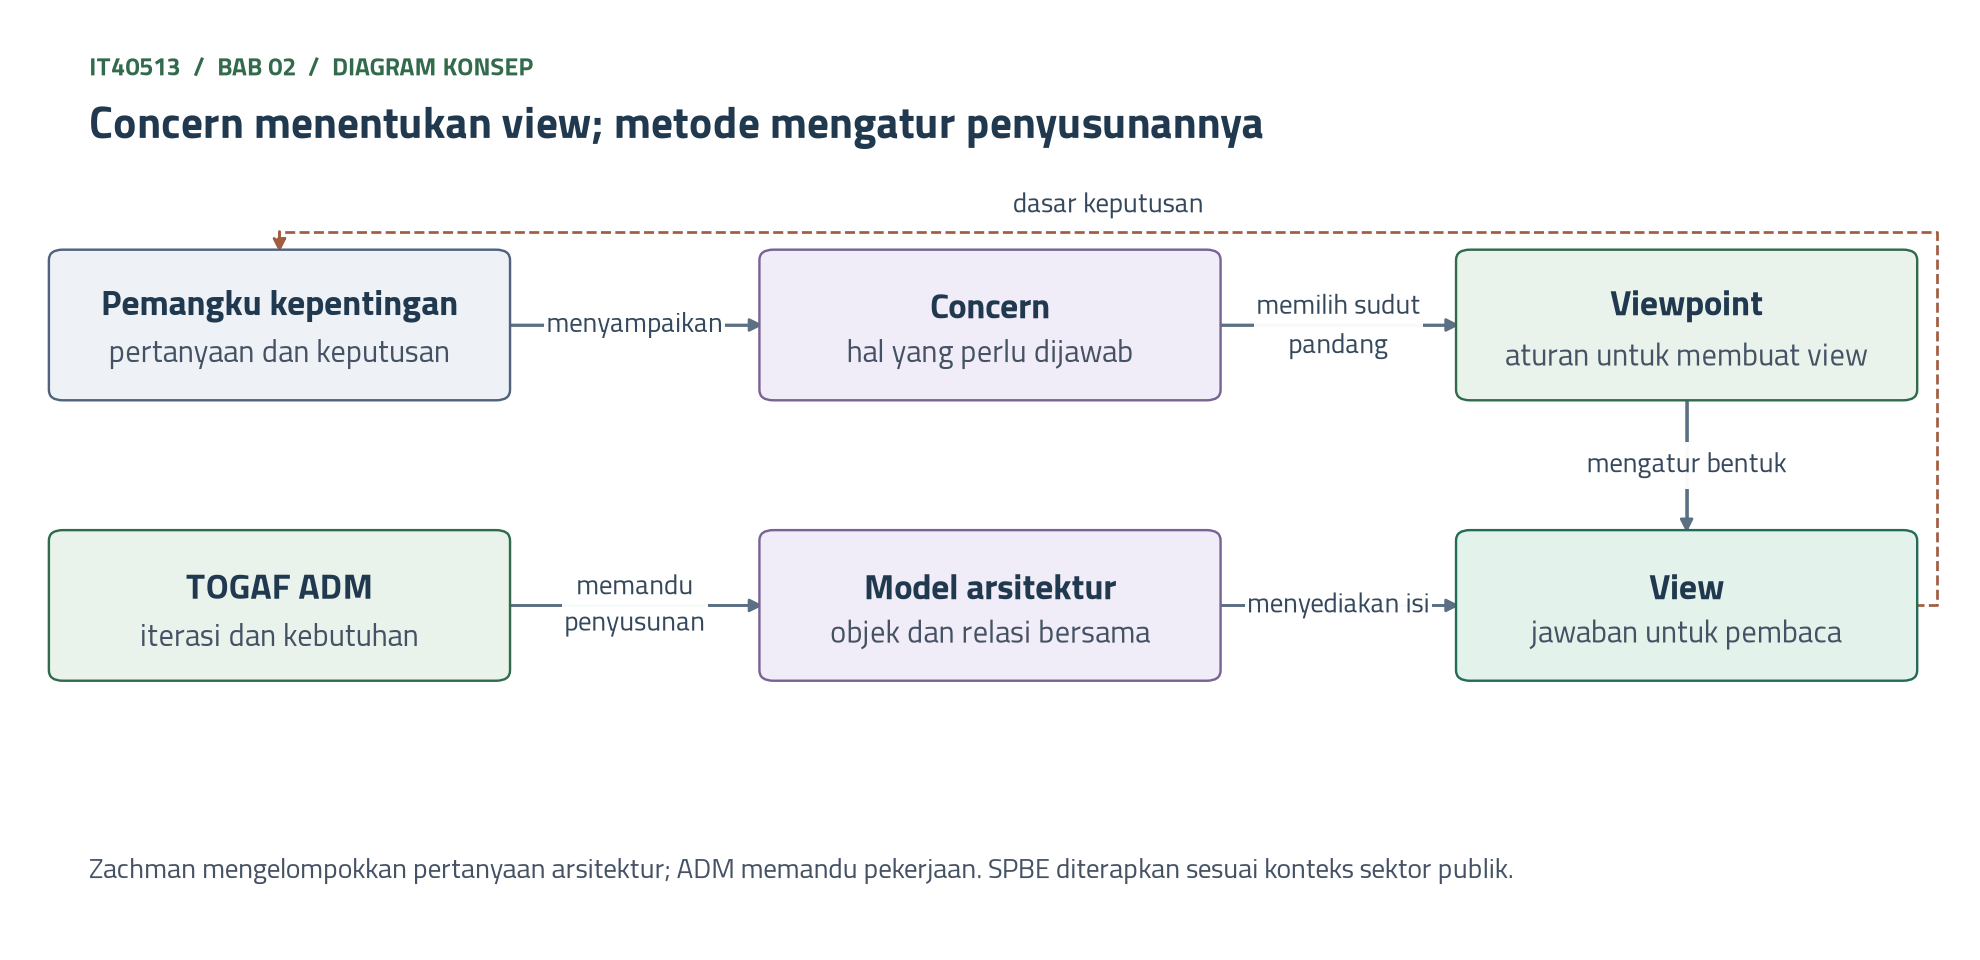
\includegraphics[width=0.96\textwidth,height=0.77\textheight,keepaspectratio]{../../figures/ch02-diagram-konsep.png}
  \label{fig:session02-ilustrasi-bab}
\end{frame}

\section{Kosakata Arsitektur}

\begin{frame}{\hfill}
  \centering
  \Huge{\textbf{Kosakata Arsitektur}}
\end{frame}

\begin{frame}{{\Large Stakeholder, Concern, View, Viewpoint}}
  \vspace{6pt}
  \small
  \begin{itemize}
    \item ISO/IEC/IEEE 42010:2022 mengatur isi minimum deskripsi arsitektur, bukan cara merancangnya.
          Arsitektur tetap ada walaupun tidak ditulis, tetapi yang dapat diperiksa hanya deskripsinya.
    \item Pemangku kepentingan (\textit{stakeholder}): orang, kelompok, atau organisasi yang
          berkepentingan atas entitas yang dikaji.
    \item \textit{Concern}: kepentingan atau pertanyaan terhadap entitas itu, misalnya biaya atau waktu
          tunggu.
    \item \textit{View}: bagian deskripsi arsitektur yang menjawab \textit{concern} tertentu.
    \item \textit{Viewpoint}: aturan untuk membuat dan membaca sebuah \textit{view}.
  \end{itemize}
\end{frame}

\begin{frame}{{\Large Setiap View Menjawab Concern}}
  \centering
  \eadiagram{../../figures/ch02-konsep-42010.tex}
\end{frame}

\begin{frame}{{\Large View dan Viewpoint: Contoh}}
  \vspace{6pt}
  \small
  \begin{itemize}
    \item Analogi: gedung satu, gambarnya banyak. Setiap gambar adalah \textit{view}. Simbol, skala, dan
          legenda baku adalah \textit{viewpoint}.
    \item Direktur Keuangan bertanya biaya integrasi per tahun. \textit{View}-nya tabel biaya per
          antarmuka selama tiga tahun, bukan diagram server setebal 40 halaman.
    \item Dokter di Bogor bertanya riwayat alergi pasien dari Jakarta. Misalkan kini lewat telepon,
          dengan tunggu 15 sampai 30 menit. \textit{View}-nya alur informasi lintas lima rumah sakit.
    \item \textit{Viewpoint} bersifat umum dan dapat dipakai ulang, \textit{view} bersifat khusus.
    \item ArchiMate menyediakan \textit{viewpoint} siap pakai. Bab 4 memakainya.
  \end{itemize}
\end{frame}

\begin{frame}{{\Large Matriks Kekuasaan dan Kepentingan}}
  \centering
  {\small Kekuasaan: kemampuan menyetujui, menghentikan, atau mendanai. Kepentingan: seberapa besar
  pekerjaan arsitektur mengubah keadaan pihak itu.\par}
  \vspace{4pt}
  \eadiagram{../../figures/ch02-matriks-pemangku.tex}
\end{frame}

\begin{frame}{{\Large Kasus: Siapa Berkepentingan?}}
  \begin{block}{Kasus Medikara Health}
    \small
    \begin{itemize}
      \item 36 fasilitas: 5 rumah sakit, 18 klinik pratama, 1 laboratorium rujukan, 12 apotek.
      \item Daftar disusun dari bagan organisasi, kontrak pihak luar, dan regulator yang mengirim aturan
            dalam tiga tahun terakhir. Hasilnya sepuluh kelompok.
      \item ``Sistem yang lebih baik'' bukan \textit{concern}. ``Berapa aplikasi yang harus dibuka untuk
            mendaftarkan satu pasien?'' adalah \textit{concern}.
      \item BPJS Kesehatan dan Kementerian Kesehatan tidak menyusun cetak biru, tetapi aturannya membatasi
            pilihan arsitektur.
      \item Insiden kebocoran data 2025 menjadikan \textit{concern} vendor perlu dicatat.
    \end{itemize}
  \end{block}
\end{frame}

\begin{frame}{{\Large Concern Pemangku Kepentingan (1/2)}}
  \footnotesize
  \begin{tabularx}{\textwidth}{>{\raggedright\arraybackslash}p{2.3cm}
      >{\raggedright\arraybackslash}X >{\raggedright\arraybackslash}p{3.7cm}}
    \hline
    \textbf{Pemangku kepentingan} & \textbf{\textit{Concern} utama} & \textbf{\textit{View} yang menjawab} \\
    \hline
    Direksi & Apakah ``Satu Pasien, Satu Rekam Medis'' tercapai pada 2030, dan berapa biayanya? & Peta jalan satu halaman dengan biaya per tahun \\
    \hline
    Direktur Keuangan & Berapa biaya integrasi per tahun, dan integrasi mana yang paling mahal? & Tabel biaya per antarmuka dan trennya \\
    \hline
    Kepala rumah sakit & Apakah antrean berkurang tanpa menghilangkan keleluasaan lokal? & \textit{Value stream} rawat jalan dengan waktu tunggu \\
    \hline
    Dokter dan komite medik & Apakah riwayat pasien dari rumah sakit lain dapat dibuka saat pemeriksaan? & Alur informasi pasien lintas rumah sakit \\
    \hline
    Petugas pendaftaran & Berapa aplikasi yang harus dibuka untuk satu pasien? & Peta aplikasi per tahap pendaftaran \\
    \hline
  \end{tabularx}
\end{frame}

\begin{frame}{{\Large Concern Pemangku Kepentingan (2/2)}}
  \footnotesize
  \begin{tabularx}{\textwidth}{>{\raggedright\arraybackslash}p{2.3cm}
      >{\raggedright\arraybackslash}X >{\raggedright\arraybackslash}p{3.7cm}}
    \hline
    \textbf{Pemangku kepentingan} & \textbf{\textit{Concern} utama} & \textbf{\textit{View} yang menjawab} \\
    \hline
    Pasien & Apakah data pribadi aman, dan apakah identitas tidak perlu diisi ulang? & Alur data pribadi dan titik persetujuan \\
    \hline
    BPJS Kesehatan & Apakah klaim dikirim lengkap, tepat waktu, dan sesuai ketentuan? & Alur klaim dari layanan sampai pengajuan \\
    \hline
    Kementerian Kesehatan & Apakah data layanan terkirim ke SATUSEHAT sesuai standar yang ditetapkan? & Peta antarmuka ke SATUSEHAT \\
    \hline
    Kepala TI & Berapa integrasi \textit{point-to-point} yang ada, dan siapa yang punya akses ke data pasien? & Diagram integrasi dan matriks peran akses \\
    \hline
    Vendor & Bagian kontrak mana yang berubah, dan kapan? & Status tiap aplikasi di peta jalan \\
    \hline
  \end{tabularx}
\end{frame}

\section{TOGAF dan ADM}

\begin{frame}{\hfill}
  \centering
  \Huge{\textbf{TOGAF dan ADM}}
\end{frame}

\begin{frame}{{\Large Susunan TOGAF Standard Edisi Ke-10}}
  \scriptsize
  \begin{tabularx}{\textwidth}{>{\raggedright\arraybackslash}p{2.0cm}
      >{\raggedright\arraybackslash}p{4.3cm} >{\raggedright\arraybackslash}X}
    \hline
    \textbf{Bagian} & \textbf{Dokumen} & \textbf{Isi pokok} \\
    \hline
    \textit{Fundamental Content} & \textit{Introduction and Core Concepts} & Pengertian EA, konsep inti, istilah, dan cara membaca standar \\
    \hline
     & \textit{Architecture Development Method} & Fase ADM beserta tujuan, langkah, masukan, dan luarannya \\
    \hline
     & \textit{ADM Techniques} & Manajemen pemangku kepentingan, \textit{gap analysis}, manajemen risiko, serta alternatif dan \textit{tradeoff} \\
    \hline
     & \textit{Applying the ADM} & Iterasi, gaya arsitektur, dan pembagian lanskap arsitektur \\
    \hline
     & \textit{Architecture Content} & Kerangka isi, produk kerja, \textit{Enterprise Continuum}, dan \textit{Architecture Repository} \\
    \hline
     & \textit{Enterprise Architecture Capability and Governance} & Membangun kapabilitas arsitektur, tata kelola, dan \textit{architecture board} \\
    \hline
    \textit{Series Guides} & Contoh: arsitektur bisnis, keamanan, data dan informasi, metode lincah, model referensi pemerintahan & Panduan menyesuaikan isi inti untuk topik atau konteks tertentu \\
    \hline
  \end{tabularx}

  \vspace{6pt}
  \small Pembaruan Juni 2025 memasukkan \textit{Technical Corrigendum} 1 tanpa mengubah susunan ini.
\end{frame}

\begin{frame}{{\Large Deliverable, Artefak, Building Block}}
  \scriptsize
  \begin{tabularx}{\textwidth}{>{\raggedright\arraybackslash}p{3.0cm}
      >{\raggedright\arraybackslash}p{4.3cm} >{\raggedright\arraybackslash}X}
    \hline
    \textbf{Istilah} & \textbf{Ciri} & \textbf{Contoh Medikara} \\
    \hline
    \textit{Deliverable} & Disepakati, ditinjau formal, disetujui & \textit{Statement of Architecture Work} yang ditandatangani direksi \\
    \hline
    Artefak: katalog & Daftar unsur sejenis & Katalog aplikasi di 36 fasilitas \\
    \hline
    Artefak: matriks & Hubungan antara dua daftar & Matriks aplikasi lawan kapabilitas bisnis \\
    \hline
    Artefak: diagram & Gambar susunan dan hubungan & Diagram integrasi SIMRS, ERP, Medikara+, BPJS Kesehatan, dan SATUSEHAT \\
    \hline
    \textit{Architecture building block} & Kebutuhan yang dapat dipakai ulang, belum terikat produk & Layanan identitas pasien tunggal untuk seluruh fasilitas \\
    \hline
    \textit{Solution building block} & Produk atau komponen nyata & Produk pengelola identitas pasien yang dipilih pada Bab 9 \\
    \hline
  \end{tabularx}

  \vspace{6pt}
  \small \textit{Enterprise Continuum} mengelompokkan arsitektur dari yang paling umum sampai paling
  khusus. \textit{Architecture Repository} menyimpan seluruh hasil kerja.
\end{frame}

\begin{frame}{{\Large Siklus ADM}}
  \centering
  \eadiagram{../../figures/ch02-siklus-adm.tex}
\end{frame}

\begin{frame}{{\Large Fase ADM dan Pertemuan (1/2)}}
  \scriptsize
  \begin{tabularx}{\textwidth}{>{\raggedright\arraybackslash}p{3.0cm}
      >{\raggedright\arraybackslash}X >{\raggedright\arraybackslash}X
      >{\raggedright\arraybackslash}p{1.6cm}}
    \hline
    \textbf{Fase} & \textbf{Pertanyaan yang dijawab} & \textbf{Luaran utama} & \textbf{Pertemuan} \\
    \hline
    \textit{Preliminary} & Bagaimana organisasi akan bekerja dengan arsitektur? & Kerangka yang disesuaikan, prinsip arsitektur & 1, 3 \\
    \hline
    A. \textit{Architecture Vision} & Apa ruang lingkupnya, siapa yang terlibat, dan apa tujuannya? & \textit{Statement of Architecture Work}, visi arsitektur, rencana komunikasi & 2, 3 \\
    \hline
    B. \textit{Business Architecture} & Kapabilitas dan proses apa yang ada dan yang dibutuhkan? & Bagian bisnis dari \textit{Architecture Definition Document} & 5, 8 \\
    \hline
    C. \textit{Information Systems Architectures} & Data dan aplikasi apa yang ada dan yang dibutuhkan? & Bagian data dan aplikasi dari dokumen yang sama & 6, 7, 9 \\
    \hline
    D. \textit{Technology Architecture} & Platform dan infrastruktur apa yang ada dan yang dibutuhkan? & Bagian teknologi dan spesifikasi kebutuhan arsitektur & 7, 10 \\
    \hline
  \end{tabularx}
\end{frame}

\begin{frame}{{\Large Fase ADM dan Pertemuan (2/2)}}
  \scriptsize
  \begin{tabularx}{\textwidth}{>{\raggedright\arraybackslash}p{3.0cm}
      >{\raggedright\arraybackslash}X >{\raggedright\arraybackslash}X
      >{\raggedright\arraybackslash}p{1.6cm}}
    \hline
    \textbf{Fase} & \textbf{Pertanyaan yang dijawab} & \textbf{Luaran utama} & \textbf{Pertemuan} \\
    \hline
    E. \textit{Opportunities and Solutions} & Paket kerja dan arsitektur transisi apa yang dibutuhkan? & Peta jalan awal dan arsitektur transisi & 11, 12 \\
    \hline
    F. \textit{Migration Planning} & Bagaimana urutan, biaya, dan manfaat tiap langkah? & Rencana implementasi dan migrasi & 12, 13 \\
    \hline
    G. \textit{Implementation Governance} & Apakah proyek berjalan sesuai arsitektur? & Kontrak arsitektur dan penilaian kepatuhan & 14 \\
    \hline
    H. \textit{Architecture Change Management} & Perubahan apa yang cukup besar untuk memulai siklus baru? & Permintaan perubahan & 14 \\
    \hline
    Manajemen Kebutuhan & Bagaimana kebutuhan baru ditangani sepanjang siklus? & Penilaian dampak kebutuhan & semua \\
    \hline
  \end{tabularx}

  \vspace{6pt}
  \small Pertemuan 4 tidak muncul, karena isinya bahasa pemodelan yang dipakai di fase B sampai D.
\end{frame}

\begin{frame}{{\Large Iterasi dan Urutan Kerja}}
  \small
  \begin{itemize}
    \item Empat lingkaran iterasi: kapabilitas arsitektur (\textit{Preliminary} dan A), pengembangan
          arsitektur (B, C, dan D), perencanaan transisi (E dan F), tata kelola arsitektur (G dan H).
    \item Misalkan di tengah fase C Kementerian Kesehatan menambah jenis data SATUSEHAT. Kebutuhan masuk
          ke Manajemen Kebutuhan, lalu tim kembali ke fase C.
    \item Misalkan Medikara menjajaki satu apotek daring: siklus pendek tiga bulan pada fase A, B, dan C.
    \item Mata kuliah ini memakai \textit{baseline first}: masalah nyata dipahami sebelum merancang.
    \item Risikonya memotret terlalu lama, sehingga C2 dibatasi empat pertemuan.
  \end{itemize}
\end{frame}

\begin{frame}{{\Large Kasus: Tonggak pada Siklus ADM}}
  \begin{block}{Kasus Medikara Health}
    \small
    \begin{itemize}
      \item C1 Konteks dan Strategi (Pertemuan 1 sampai 3): \textit{Preliminary} dan A.
      \item C2 Kondisi Saat Ini (Pertemuan 4 sampai 7): B, C, dan D untuk \textit{baseline}.
      \item C3 Kondisi Target (Pertemuan 8 sampai 11): B, C, dan D untuk target, lalu memulai E lewat
            \textit{gap analysis}.
      \item C4 Peta Jalan dan Tata Kelola (Pertemuan 12 sampai 14): menyelesaikan E dan F, lalu merancang
            G dan H.
      \item Di Medikara yang sesungguhnya, G dan H berjalan bertahun-tahun. Di kelas keduanya hanya
            dirancang.
    \end{itemize}
  \end{block}
\end{frame}

\section{Zachman Framework}

\begin{frame}{\hfill}
  \centering
  \Huge{\textbf{Zachman Framework}}
\end{frame}

\begin{frame}{{\Large Zachman: Ontologi, Bukan Metodologi}}
  \vspace{6pt}
  \small
  \begin{itemize}
    \item Makalah 1987 memuat tiga kolom. Sowa dan Zachman melengkapinya menjadi enam kolom: apa,
          bagaimana, di mana, siapa, kapan, dan mengapa.
    \item Enam baris menyatakan sudut pandang, dari eksekutif yang menetapkan cakupan sampai organisasi
          yang sedang berjalan.
    \item Analogi: lemari arsip dengan 36 laci berlabel. Laci kosong terlihat, urutan membuatnya tidak.
    \item ADM menghasilkan artefak, dan Zachman memeriksa apakah artefak itu menutup sel yang penting.
    \item Godaan mengisi seluruh 36 sel perlu dilawan: sel tanpa pembaca hanya menambah dokumen yang
          tidak terpelihara.
  \end{itemize}
\end{frame}

\begin{frame}{{\Large Zachman sebagai Daftar Periksa}}
  \centering
  % Huruf diperkecil hanya di slide ini: font tema lebih lebar daripada font modul,
  % sehingga label baris dan legenda bertumpuk pada ukuran bawaan gambar.
  \begingroup
    \renewcommand{\scriptsize}{\fontsize{6.5}{7.5}\selectfont}
    \renewcommand{\tiny}{\fontsize{5}{6}\selectfont}
    \eadiagram{../../figures/ch02-zachman-medikara.tex}
  \endgroup
\end{frame}

\begin{frame}{{\Large Kasus: Lemari Arsip Kosong di Tengah}}
  \begin{block}{Kasus Medikara Health}
    \small
    \begin{itemize}
      \item Misalkan dokumen diinventarisasi. Dari 30 sel pada baris 1 sampai 5: 12 sel terkini, 11 sel
            sebagian atau usang, dan 7 sel kosong.
      \item Baris 1 hampir lengkap, dan baris 5 juga lengkap.
      \item Lima dari tujuh sel kosong berada di baris 3, yang menghubungkan keputusan direksi dengan
            konfigurasi teknis.
      \item Sel peta integrasi kosong sejalan dengan biaya integrasi tinggi. Sel matriks peran akses
            kosong sejalan dengan temuan audit.
      \item Membiarkan sel kosong adalah keputusan sadar, lengkap dengan alasannya.
    \end{itemize}
  \end{block}
\end{frame}

\section{Arsitektur SPBE}

\begin{frame}{\hfill}
  \centering
  \Huge{\textbf{Arsitektur SPBE}}
\end{frame}

\begin{frame}{{\Large Arsitektur SPBE dan Statusnya}}
  \small
  \begin{itemize}
    \item Peraturan Presiden (Perpres) 95/2018: kerangka dasar yang mendeskripsikan integrasi proses
          bisnis, data dan informasi, infrastruktur, aplikasi, dan keamanan SPBE.
    \item Tiga tingkat: nasional, instansi pusat, dan pemerintah daerah. Disusun untuk lima tahun, lalu
          ditinjau pada paruh waktu dan tahun terakhir.
    \item Perpres 132/2022: Arsitektur SPBE Nasional periode 2020 sampai 2024.
    \item Perpres 82/2023: Aplikasi SPBE Prioritas. Perpres 83/2025: Komite Percepatan Transformasi
          Digital Pemerintah. Peraturan Menteri PANRB 8/2026: evaluasi kinerja.
    \item Status per 30 Oktober 2026: Perpres 95/2018 masih berlaku, revisinya masih disusun. Status ini
          diperiksa ulang di basis data peraturan resmi.
  \end{itemize}
\end{frame}

\begin{frame}{{\Large Enam Domain SPBE, Empat Domain TOGAF}}
  \centering
  \eadiagram{../../figures/ch02-domain-spbe-togaf.tex}

  \vspace{4pt}
  {\small Artefak layanan dan keamanan dijadwalkan eksplisit di fase B sampai D. Keamanan dikoordinasi
  lembaga di bidang keamanan siber.\par}
\end{frame}

\begin{frame}{{\Large Kasus: Mengapa Swasta Membaca SPBE?}}
  \begin{block}{Kasus Medikara Health}
    \small
    \begin{itemize}
      \item Medikara perusahaan swasta, sehingga tidak wajib menyusun Arsitektur SPBE.
      \item Perpres 95/2018 menyebut pelaku usaha sebagai salah satu Pengguna SPBE (Pasal 1 angka 26).
      \item Data layanan dikirim ke SATUSEHAT dengan standar HL7 FHIR, dan klaim dikirim ke BPJS
            Kesehatan.
      \item Perubahan format SATUSEHAT mengubah antarmuka kelima SIMRS. Perubahan aturan klaim mengubah
            proses di loket.
      \item Arsitek memantau Arsitektur SPBE dan Peraturan Menteri Kesehatan 24/2022.
    \end{itemize}
  \end{block}
\end{frame}

\section{Penyesuaian dan Aktivitas}

\begin{frame}{\hfill}
  \centering
  \Huge{\textbf{Penyesuaian dan\\Aktivitas}}
\end{frame}

\begin{frame}{{\Large Menyesuaikan Kerangka untuk Organisasi}}
  \vspace{6pt}
  \small
  \begin{itemize}
    \item Fase \textit{Preliminary} menghasilkan \textit{Tailored Architecture Framework}: keputusan
          tertulis tentang fase, teknik, dan artefak yang dipakai.
    \item Kotusev: 27 organisasi, 24 artefak umum yang terbukti berguna. Organisasi memakai campuran,
          bukan seluruh daftar.
    \item Misalkan tim Medikara tiga orang melayani 36 fasilitas, lalu memilih 12 artefak.
    \item Analogi: resep 50 porsi untuk delapan orang. Takaran dikecilkan, langkah yang menjaga makanan
          aman tidak dilewati.
    \item Tanda kebablasan: \textit{concern} pemain kunci tidak terjawab, atau keputusan besar tidak dapat
          ditelusuri.
  \end{itemize}
\end{frame}

\begin{frame}{{\Large Artefak Minimum Cetak Biru Capstone}}
  \scriptsize
  \begin{tabularx}{\textwidth}{>{\raggedright\arraybackslash}X
      >{\raggedright\arraybackslash}p{1.9cm} >{\raggedright\arraybackslash}p{3.4cm}
      >{\raggedright\arraybackslash}p{1.6cm}}
    \hline
    \textbf{Artefak} & \textbf{Fase ADM} & \textbf{Bentuk} & \textbf{Pertemuan} \\
    \hline
    Peta pemangku kepentingan dan \textit{concern} & A & Matriks dan diagram & 2 \\
    \hline
    \textit{Statement of Architecture Work} & A & \textit{Deliverable} & 2 \\
    \hline
    Prinsip arsitektur & \textit{Preliminary} & Katalog & 3 \\
    \hline
    Visi arsitektur & A & \textit{Deliverable} & 3 \\
    \hline
    Model ArchiMate berlapis & B sampai D & Diagram & 4 \\
    \hline
    \textit{Capability map} dan \textit{heatmap} & B & Diagram & 5, 8 \\
    \hline
    Matriks CRUD (\textit{Create, Read, Update, Delete}) & C & Matriks & 6 \\
    \hline
    Katalog aplikasi dan diagram integrasi & C, D & Katalog dan diagram & 7, 9 \\
    \hline
    Catatan keputusan arsitektur & D & Dokumen singkat & 10 \\
    \hline
    Matriks gap dan paket kerja & E & Matriks & 11 \\
    \hline
    Peta jalan dan rencana migrasi & E, F & Diagram dan \textit{deliverable} & 12 \\
    \hline
    Rancangan tata kelola arsitektur & G, H & \textit{Deliverable} & 14 \\
    \hline
  \end{tabularx}
\end{frame}

\begin{frame}{{\Large Aktivitas: Peran dan Langkah}}
  \vspace{6pt}
  \small
  \begin{itemize}
    \item Analis bisnis memimpin identifikasi pemangku kepentingan. Analis teknologi melengkapi
          \textit{concern} teknis dan regulasi.
    \item Pemodel memilih fase ADM dan artefak minimum. Koordinator merangkum ruang lingkup.
    \item Daftarkan minimal 10 kelompok. Beri nilai kekuasaan dan kepentingan skala 1 sampai 5, dengan
          nilai 3 ke atas dianggap tinggi.
    \item Tulis \textit{concern} sebagai pertanyaan, tentukan \textit{view}, lalu tetapkan ruang lingkup.
    \item Rangkai hasil dalam \textit{Statement of Architecture Work} dua sampai tiga halaman.
  \end{itemize}
\end{frame}

\begin{frame}{{\Large Contoh Statement of Architecture Work}}
  \scriptsize
  \begin{tabularx}{\textwidth}{>{\raggedright\arraybackslash}p{2.6cm}
      >{\raggedright\arraybackslash}X}
    \hline
    \textbf{Komponen} & \textbf{Isi untuk Medikara} \\
    \hline
    Latar belakang & Strategi ``Satu Pasien, Satu Rekam Medis''; insiden kebocoran data lewat vendor pada 2025; temuan audit kontrol akses; antrean panjang; biaya integrasi tinggi \\
    \hline
    Unit organisasi & 5 rumah sakit, 18 klinik pratama, 1 laboratorium rujukan, 12 apotek, dan kantor pusat \\
    \hline
    Horizon waktu & Kondisi saat ini per 2026, kondisi target 2030, dengan arsitektur transisi di antaranya \\
    \hline
    Domain & Bisnis, data, aplikasi, dan teknologi; keamanan dan kepatuhan sebagai \textit{concern} lintas domain \\
    \hline
    Batasan & Misalkan ERP keuangan tidak diganti pada siklus ini; hanya antarmukanya yang ditinjau \\
    \hline
    Peran & Sponsor: Direktur Utama; pemilik arsitektur: kepala TI; tim: koordinator, analis bisnis, analis teknologi, pemodel \\
    \hline
    Kriteria penerimaan & Setiap \textit{concern} pemain kunci dijawab minimal satu \textit{view}; seluruh artefak minimum tersedia pada tonggak C1 sampai C4 \\
    \hline
    Jadwal & C1 Pertemuan 3, C2 menjelang UTS, C3 Pertemuan 11, C4 menjelang UAS \\
    \hline
    Persetujuan & Ditandatangani sponsor dan pemilik arsitektur \\
    \hline
  \end{tabularx}
\end{frame}

\begin{frame}{{\Large Luaran C1 dan Kriteria Penilaian}}
  \footnotesize
  \begin{tabularx}{\textwidth}{>{\raggedright\arraybackslash}p{5.0cm} r
      >{\raggedright\arraybackslash}X}
    \hline
    \textbf{Kriteria} & \textbf{Bobot} & \textbf{Ciri hasil yang baik} \\
    \hline
    Kelengkapan pemangku kepentingan & 25\% & Pihak luar dan regulator tercatat; penempatan di matriks disertai alasan \\
    \hline
    Ketajaman \textit{concern} & 25\% & Ditulis sebagai pertanyaan yang dapat dijawab dengan data \\
    \hline
    Kejelasan ruang lingkup & 30\% & Unit, horizon waktu, domain, dan batasan tertulis eksplisit \\
    \hline
    Kesesuaian artefak dan fase & 20\% & Setiap artefak yang ditambah atau dibuang punya alasan \\
    \hline
  \end{tabularx}

  \vspace{8pt}
  \small Luaran: peta pemangku kepentingan dan \textit{Statement of Architecture Work}. Templat tersedia
  di \berkas{sources/chapter02/README.md}.
\end{frame}

\begin{frame}{{\Large Ringkasan}}
  \vspace{6pt}
  \small
  \begin{itemize}
    \item Pemangku kepentingan memiliki \textit{concern}, \textit{viewpoint} membingkainya, dan
          \textit{view} menjawabnya.
    \item Inti TOGAF adalah ADM: \textit{Preliminary}, fase A sampai H, dan Manajemen Kebutuhan di
          tengah.
    \item Zachman adalah ontologi, ADM adalah metode. Pada Medikara, 7 dari 30 sel kosong.
    \item Arsitektur SPBE: tiga tingkat, lima tahun, enam domain. Layanan dan keamanan ditangani secara
          eksplisit.
    \item Pesan utama: kerangka kerja adalah alat, bukan tujuan. Penyesuaian yang baik membuang artefak
          tanpa pembaca dan menjaga setiap keputusan dapat ditelusuri.
  \end{itemize}
\end{frame}

\begin{frame}{{\Large Latihan}}
  \vspace{6pt}
  \small
  \begin{enumerate}
    \item \textit{Concern} Direktur Keuangan dan Kepala TI: misalkan proyek layanan identitas pasien
          tunggal untuk 36 fasilitas. Tulis dua \textit{concern} tiap pihak sebagai pertanyaan, lalu
          tentukan \textit{view}-nya.
    \item Ontologi dan Metode: pilih enam artefak minimum. Tentukan sel Zachman dan fase ADM tiap
          artefak, lalu catat sel penting yang tidak terisi.
    \item Enam Domain SPBE dan Empat Domain TOGAF: misalkan rumah sakit umum daerah memakai ADM. Tentukan
          padanan TOGAF tiap domain SPBE dan cara menangani domain tanpa padanan langsung.
  \end{enumerate}
\end{frame}

\begin{frame}{{\Large Bacaan dan Berkas Pendukung}}
  \vspace{10pt}
  \begin{itemize}
    \item \href{https://www.iso.org/standard/74393.html}{\textit{Software, Systems and Enterprise: Architecture Description}}
    \item \href{https://www.opengroup.org/togaf}{\textit{The TOGAF Standard, 10th Edition (2025 Update)}}
    \item \href{https://www.vanharen.net/store/the-togafr-standard-10th-edition-a-pocket-guide-2025-update}{\textit{The TOGAF Standard, 10th Edition: A Pocket Guide, 2025 Update}}
    \item \berkas{sources/chapter02/README.md}
  \end{itemize}
\end{frame}

\end{document}
